%!TEX root = ../thesis.tex
%*******************************************************************************
%****************************** Third Chapter **********************************
%*******************************************************************************
\chapter{Requirements Elicitation}
\graphicspath{{Chapter4/Figs/Raster/}{Chapter4/Figs/}}

Background literature review in Chapter 2.1 and 2.2 has driven the direction of the project and 
provided many of the functional requirements. This chapter describes the further collection of primary 
data, and provides the list of formal user requirements.

\section{Primary Data and Analysis}
Collecting primary data from shareholders of higher education e-learning systems would be able to:
\begin{itemize}
    \item reaffirm and further develop requirements obtained from literature
    \item obtain further requirements from real world painpoints and goals
\end{itemize}

\subsection{Methodology}

[TODO]

Method: qualitative

Instrument: Why interviews?

Sample: Participants are needed who are 
\begin{itemize}
    \item Teaching staff in higher education with 10+ years of experience
    \item Student
\end{itemize}Teachers with  in Who are they? Why? Convenience Sampling. Limitation: all CS department.

An ethics submission was completed on BREO and approval granted on 21st November. 
See Appendix (TODO) for the approved participant information sheet, consent form and example questions.

A total of five interviews were conducted between December 2017 and February 2018: 
two with teaching staff and three with student representatives. See table 
\ref{table:participants-req} for a more detailed description of these participants.

\begin{table}[!h] 
    \caption{Participants in primary data collection interviews}
    \centering
    \label{table:participants-req}
    \begin{tabularx}{\textwidth}{>{\bfseries}lX}
        Participant & Characterisation\\
        \toprule
        Educator A & lecturer in higher education for over 20 years, and an experienced higher education 
        administrator\\\midrule
        Educator B & lecturer in higher education for over 20 years, with research interests 
        in e-learning interactions, effectiveness and acceptance\\\midrule
        Student C & a university course representative for 3 years, which involves collecting and 
        communicating student feedback and attending staff-student liaison meetings \\\midrule
        Student D & a university peer assisted learning leader for 2 years, helping out lower level 
        students with their academic work by facilitating peer discussions, and escalating common problems
        to academic staff in debrief sessions\\\midrule
        Student E & a university course representative for 2 years and a peer assisted learning leader 
        for 1 year\\\bottomrule
    \end{tabularx}
\end{table}

\subsection{Interview Results and Analysis}

The raw data from interviews (transcripts) were contextually analysed and grouped into problem statements (PS), 
these problem statements were then sorted into groups to produce an affinity diagram (See figure 
\ref{fig:ps-affinity}).

Below you will find the sample questions asked for each group, detailed descriptions and relevant transcript 
snippets for each problem statements. 
Any specifics regarding course, staff and event details have been anonymised.

\begin{figure}[!ht] 
    \centering    
    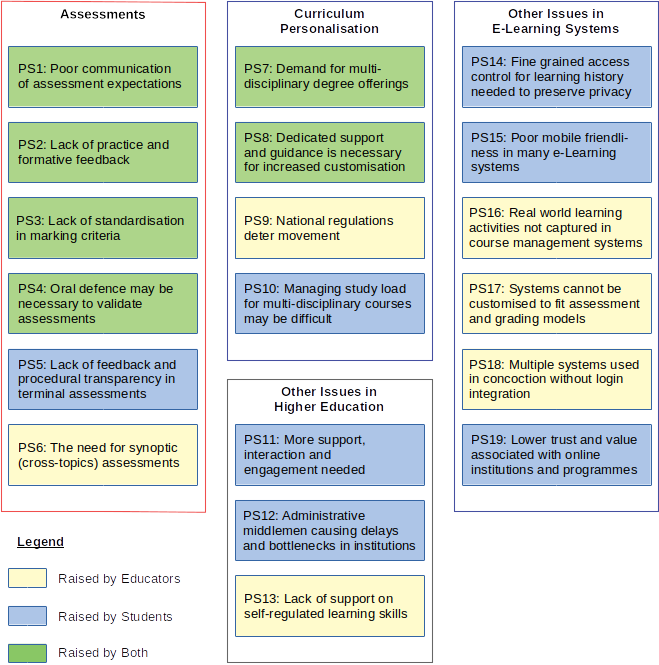
\includegraphics[width=1.0\textwidth]{ps-affinity}
    \caption[Affinity diagram for primary data]
        {Affinity diagram for problem statements devised from primary data}
    \label{fig:ps-affinity}
\end{figure}



\section{Formal Requirements}

Table \ref{table:fx-reqs} lists out the functional requirements (FR) adopted by this 
project going forward. They are related to one or more of the problem statements (PS) gathered 
above from primary data, or to the literature reviewed in Chapter 2. 

Table \ref{table:nonfx-reqs} lists the non-functional requirements (NR) adopted by this 
project going forward. They are related to one or more of the problem statements (PS) gathered, 
or to usability heuristics.

These requirements have been ranked with the MoSCoW prioritisation
framework, which specified four levels of priority: Must Have, Should Have, Could Have, and Won’t Have 
this time \citep{agile2018moscow}. The MoSCoW levels are given from mainly a system engineering perspective 
in planning the minimum viable product for the demonstrator of this project, 
and do not necessarily reflect the priorities of the stakeholders.

\begin{table}[!h] 
    \caption{Prioritised list of functional requirements for this project}
    \centering
    \label{table:fx-reqs}
    \begin{tabularx}{\textwidth}{>{\bfseries}l>{\hsize=1.5\hsize}X>{\hsize=.5\hsize}Xl}
        & Requirement Statements & Related To & MoSCoW\\
        \toprule
        FR1 & The system would store learner records on a blockchain 
        & Ch 2.2.1 (LTSA) & Must Have
        \\\midrule
        FR2 & Teachers would be able to create and edit learning resources
        & Ch 2.2.1 (LTSA) & Must Have
        \\\midrule
        FR3 & Teachers would be able to create and edit assessments
        & Ch 2.2.1 (LTSA) & Must Have
        \\\midrule
        FR4 & The system would enforce the provision of learning outcomes, knowledge required 
        and assessment goals at the creation or update of modules & Ch 2.1.1 (Transparency), 
        PS1 & Must Have
        \\\midrule
        FR5 & The system would enforce predefined assessments rules (eg. marking schemes, 
        transparent procedures and feedback) with smart contracts 
        & Ch 2.1.1 (Transparency), PS3, PS5 & Must Have
        \\\midrule
        FR6 & The system would allow teachers to configure multiple assessments and 
        formative assessments for modules & PS2 & Could Have
        \\\midrule
        FR7 & The system would require vivas (oral defences) after automated assessments & 
        PS4 & Could Have
        \\\midrule
        FR8 & The system would provide flexible configurability for grade schema & PS17
        & Could Have
        \\\midrule
        FR9 & Teachers would be able to create a customised list of courses 
        for a student, customising programme outcomes and specifications 
        & Ch 2.1.2 (Personalisation), PS7, PS9 & Must Have
        \\\midrule
        FR10 & The system should feature dedicated support channels between students, teachers 
        and other advisors 
        & PS8, PS11 & Should Have
        \\\midrule
        FR11 & Students would be able to add assessment submissions on the blockchain 
        & Figure \ref{fig:moocon_assess} (Concept)& Must Have
        \\\midrule
        FR12 & The system would be able to generate certificates on the blockchain when a course 
        has been completed & Figure \ref{fig:moocon_assess} (Concept) & Must Have
        \\\midrule
        FR13 & The system would allow students to control access to their education history 
        on the blockchain & PS14 & Should Have
        \\\midrule
        FR14 & The system would provide one login for content delivery, assessment and 
        record keeping & PS18 & Should Have
        \\\midrule
         &  \multicolumn{2}{c}{Requirements targetting PS6, PS10, PS13, PS16} & Won't Have
        \\\bottomrule
    \end{tabularx}
\end{table}

\begin{table}[!h] 
    \caption{Prioritised list of non-functional requirements for this project}
    \centering
    \label{table:nonfx-reqs}
    \begin{tabularx}{\textwidth}{>{\bfseries}l>{\hsize=1.6\hsize}X>{\hsize=.4\hsize}Xl}
        & Requirement Statements & Related To & MoSCoW
        \\\toprule
        NR1 & The client applications would have the same functionalities across devices and 
        a responsive interface & PS15 & Should Have
        \\\midrule
        NR2 & The client applications would fail safely and is error-forgiving 
        towards the user &  & Should Have
        \\\midrule
        NR3 & The client applications would notify users of relevant events on the blockchain
        network &  & Should Have
        \\\midrule
        NR4 & The system should be able to reduce administrative work & PS12 & Should Have
        \\\midrule
        NR5 & The system should be able to create more trust in online education providers 
        and programmes & PS19 & Should Have
        \\\bottomrule
    \end{tabularx}
\end{table}